
\chapter{The CMS detector owerwiew}

%rewrite
The CMS detector is a multipurpose detector at the LHC. The detector layout is outlined in Figure \ref{fig:CMS_detector}. The detector consists of various sub-parts designed to measure different properties of the collision-produced particles. The closest to the interaction point (IP) is the tracker system, which operates within a 3.8 T magnetic field. Comprising pixel and strip detectors enables precise measurement of transverse momentum and positions of charged particles. In addition, reconstruction algorithms employed in the determination of the trajectories also yield fundamental information regarding single collisions, for instance, the impact parameter, which plays a critical role in displaced vertex identification and association to tracks for further sophisticated methods such as PU mitigation and flavor tagging.

\begin{figure}[h]
    \centering
    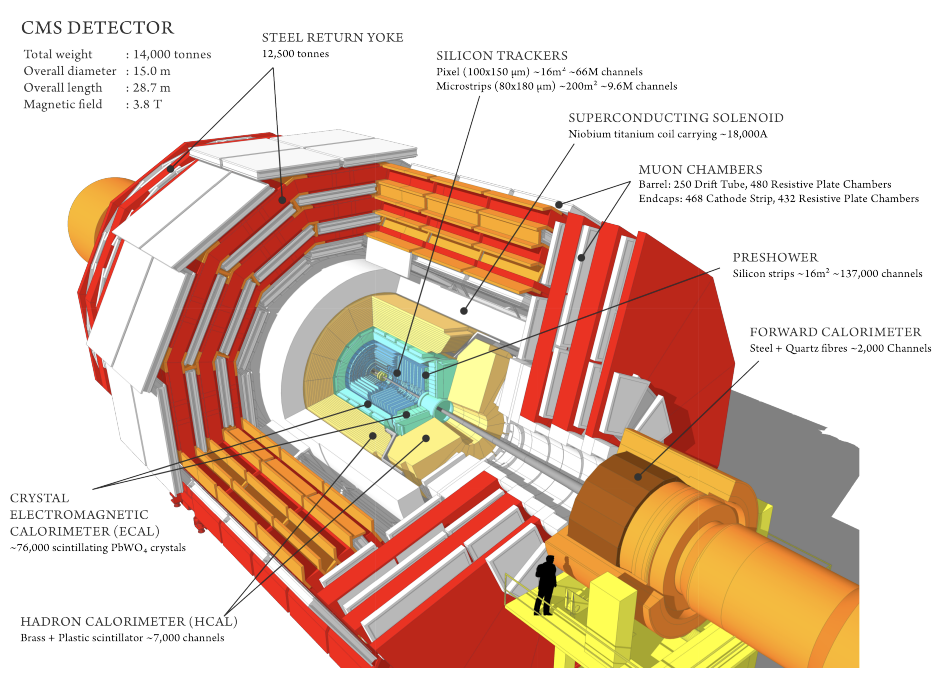
\includegraphics[width=0.9\textwidth]{images/CMS_detector.png}
    \caption{The CMS detector at the LHC \cite{Ghosh_2019}.}
    \label{fig:CMS_detector}
\end{figure}

The tracker system is followed by the electromagnetic (ECAL) and hadronic (HCAL) calorimeters. ECAL stops electromagnetically interacting particles, producing an electromagnetic shower as a result. That allows to measure the energy of these particles with high precision. HCAL has a similar principle of work but for hadrons, which are interacting strongly with absorber material. Some particles can pass calorimeters undetected, like neutrinos, for example, or just lose some energy, like muons. The presence of these particles can be detected by calculating reconstructed particles' momenta, also called missing transverse energy (MET). The calorimeters are crucial for jet reconstruction.

The outer part of the detector is the muon system, or muon chambers. Muons are distinguished by their minimal energy loss in the calorimeters and by matching tracks between the inner tracker and the muon system. Their momentum and position are measured there. Particles like neutrinos pass through the last layer of the detector without any interaction and can be detected only through MET \cite{The_CMS_Collaboration_2008, Hayrapetyan_2024}.

\section{Phase-2 Tracker Upgrade for the HL-LHC}

Phase-2 upgrade of the CMS detector is desighn to await the challenges facing the HL-LHC. Increase in luminosity by a factor of 5 and up to 200 bunch crossing collisions will expose the CMS tracking system to severe challenges, primarily due to high radiation levels and high density particle environment. The upgrade will include a new IT with a re-designed pixel detector with reduced pixel size, improved spatial resolution, and tracking capabilities. The current Phase-1 detector has pixel sizes of $100 \times 150~\mu\text{m}^2$, while the Phase-2 upgrade will include pixel sizes as small as $25 \times 100~\mu\text{m}^2$ in the barrel and $50 \times 50~\mu\text{m}^2$ in some forward regions (see Figure~\ref{fig:IT}), which supports a significant improvement in granularity \cite{thetrackergroupofthecmscollaboration2023evaluationplanarsiliconpixel, Orfanelli:2780125}.

\begin{figure}[H]
    \centering
    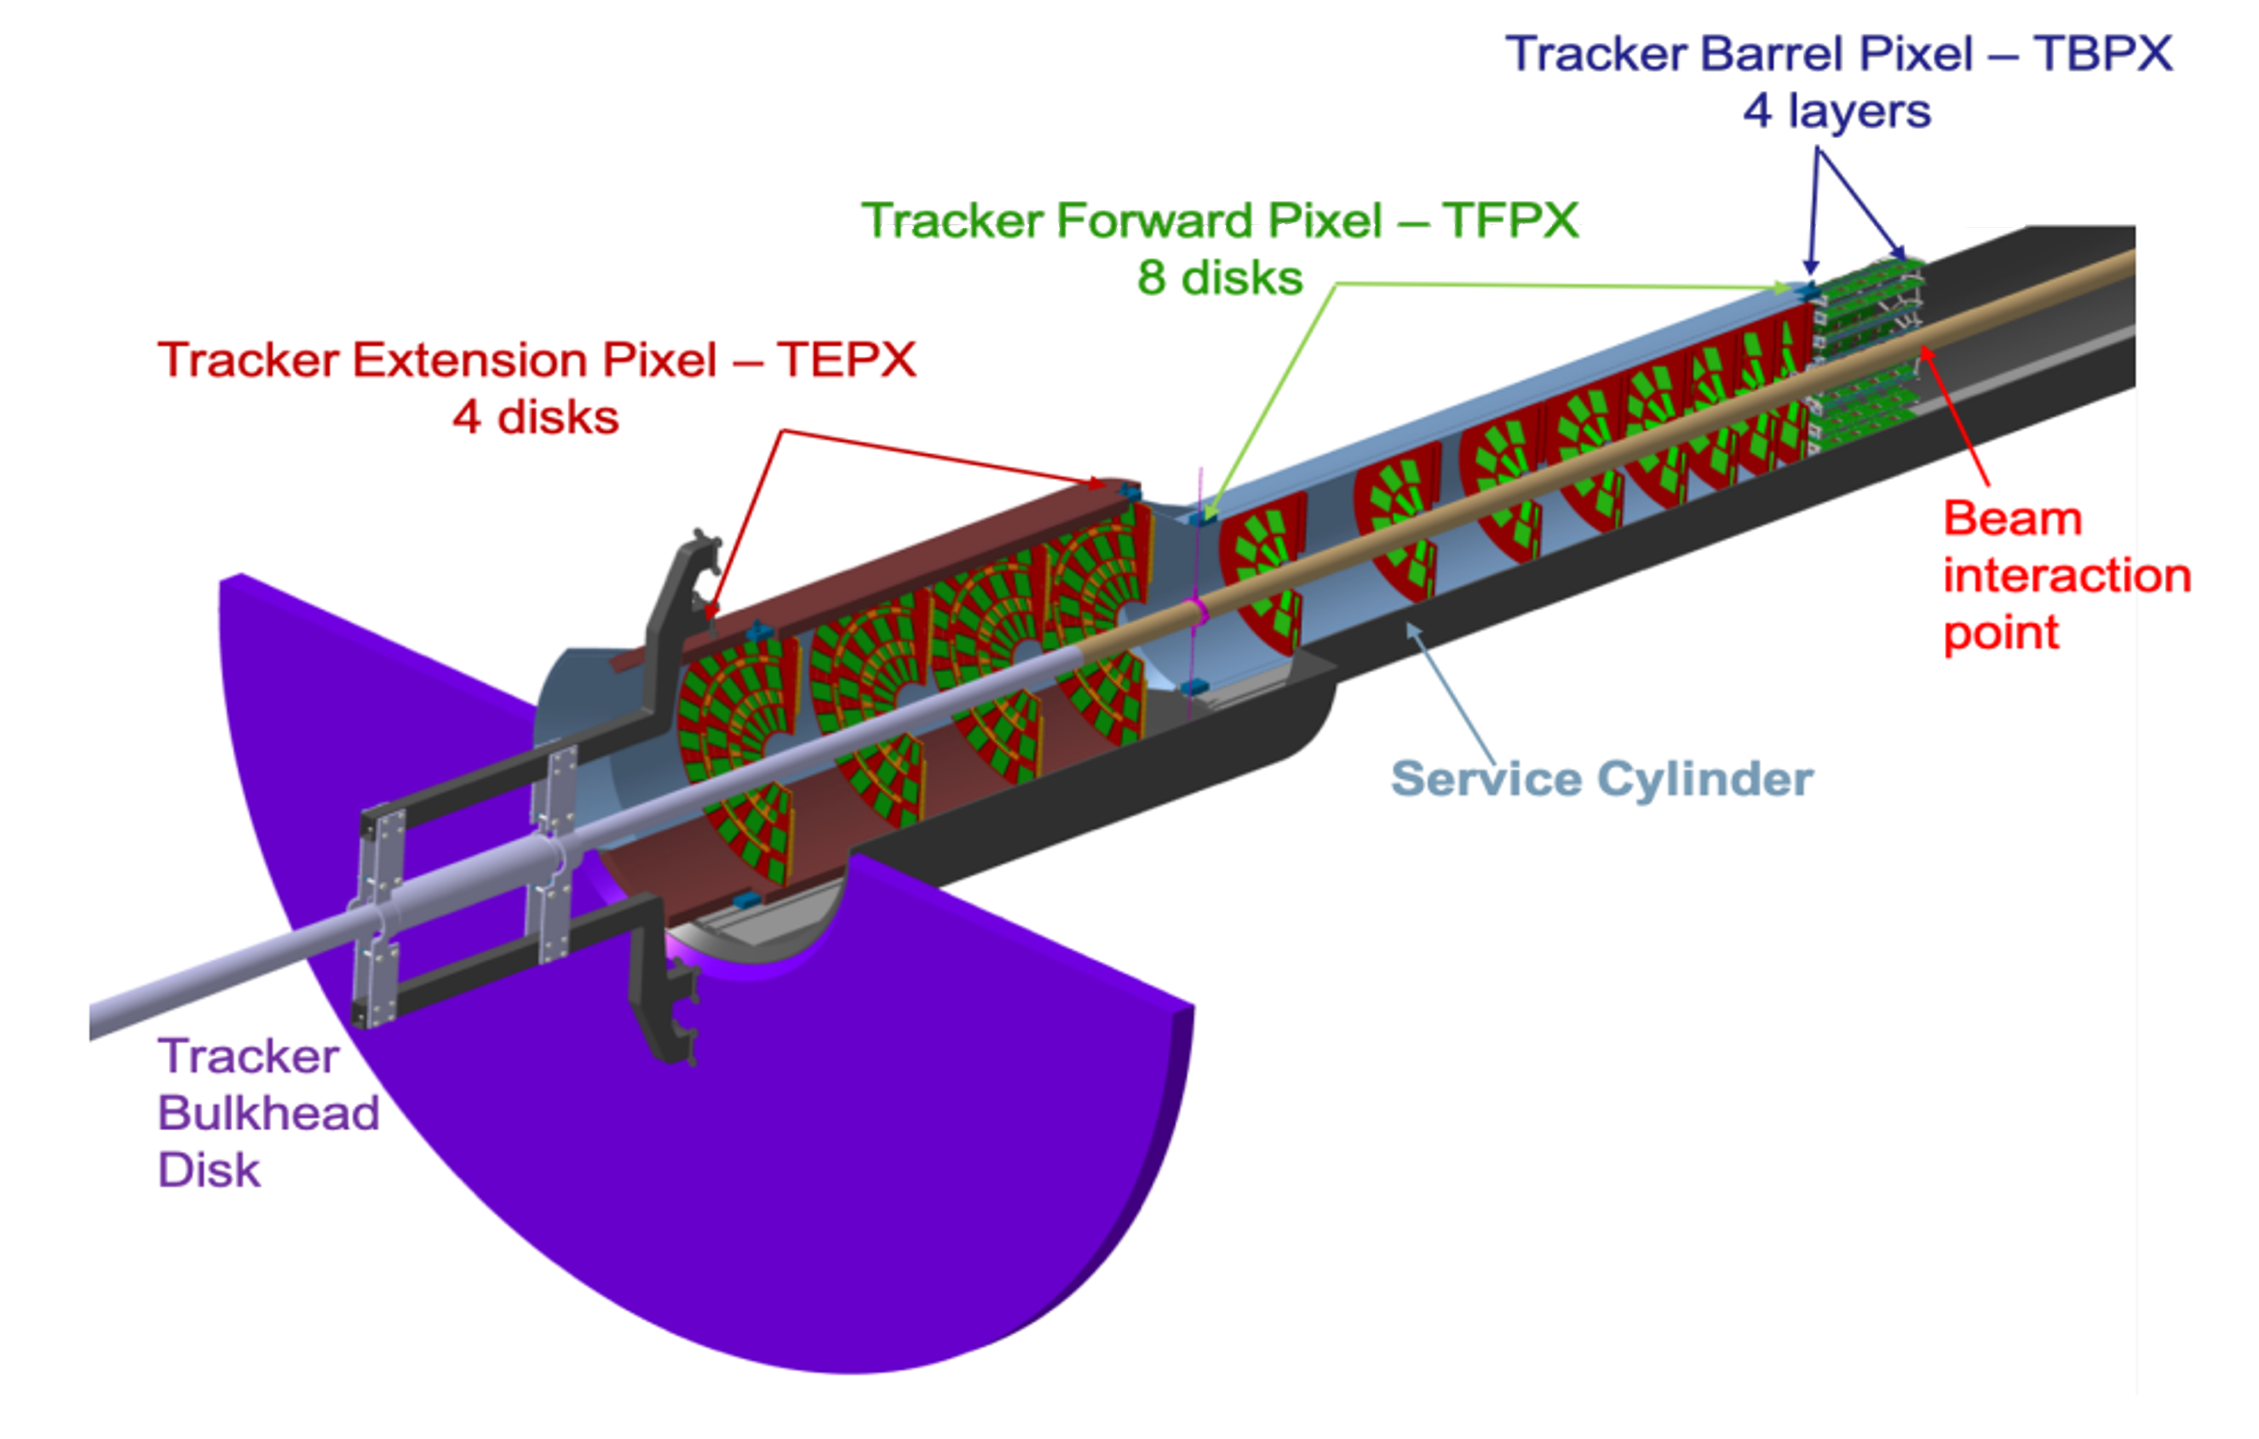
\includegraphics[width=0.8\textwidth]{images/IT.png}
    \caption{Exploded view of the CMS Phase-2 IT layout quarter, showing the Tracker Barrel Pixel (TBPX), the Tracker Forward Pixel (TFPX), and the Tracker Extension Pixel (TEPX).}
    \label{fig:IT}
\end{figure}

The Inner Tracker will consist of approximately two billion pixels, each with an area of $2500~\mu\text{m}^2$, arranged in modules with either two or four front-end readout chips, depending on their position. Two-chip modules are used in the inner barrel and the inner forward rings, while four-chip modules are employed in the outer barrel and outer forward regions, as shown in Figure~\ref{fig:tracking_layout}. This configuration enables tracking coverage up to $|\eta| \approx 4$, significantly improving the reconstruction of forward tracks and enhancing sensitivity to highly boosted or displaced signatures.

\begin{figure}[H]
    \centering
    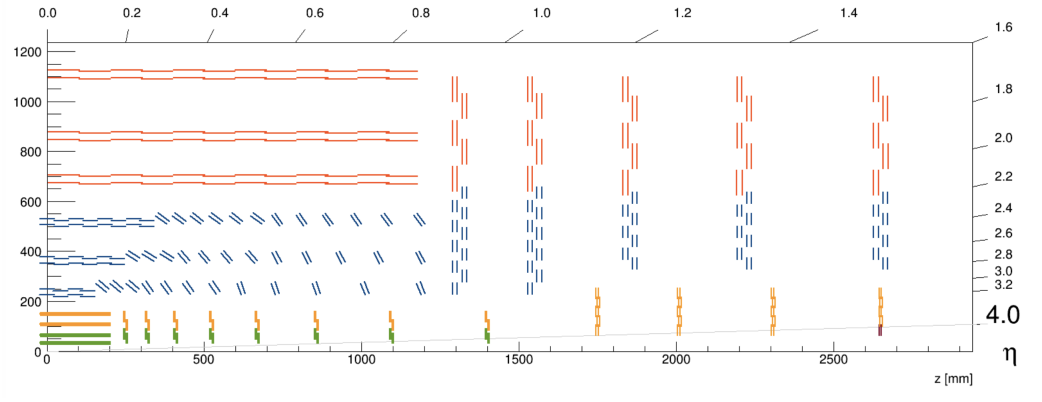
\includegraphics[width=1\textwidth]{images/tracker_layout.png}
    \caption{Sketch of one quarter of the CMS Phase-2 Tracker layout in the longitudinal ($z$--$r$) plane. Outer Tracker modules are shown in red (strip-only) and blue (pixel-strip), while Inner Tracker pixel modules are shown in green (double readout chip) and orange (quad readout chip). The $z$-axis runs along the beam direction, and the $r$-axis indicates the radial distance from the beamline. The right vertical axis shows the corresponding pseudorapidity ($\eta$) coverage, which extends up to $|\eta| \approx 4$ \cite{Outertracker}.}
    \label{fig:tracking_layout}
\end{figure}

The improved Inner Tracker is aimed at long-term functionality under severe radiation environments, with sensor modules having the ability to sustain fluences up to $2 \times 10^{16}~\text{n}_\text{eq}/\text{cm}^2$ \cite{Malik:2816244}. Moreover, it is anticipated to play a significant role in the Level-1 trigger system by providing quick tracking information essential to fast event selection. Whereas this emphasis is on the Inner Tracker, the Outer Tracker will give further coverage by utilizing strip-based 2S and PS modules, organized into six barrel layers and twelve endcap disks \cite{Outertracker}.

\section{Data Quality Monitoring of the Tracker System}

The function of the CMS detector is to reconstruct particles and events produced by proton-proton collisions. Naturally, none of the subdetectors performs ideally, and each measures physical properties with finite precision. As the Tracker system is the closest to the IP, its precise functioning is crucial to the reconstruction of primary and secondary vertices (PVs and SVs) and to obtaining better spatial resolution. It is thus imperative to ensure the optimal functioning of this system for reliable physics analyses and this needs to be supported by a strong framework for Data Quality Monitoring (DQM).


The tracker DQM infrastructure monitors the status and output of silicone pixels and strip detectors while taking frequent data. This includes checking for dead or noisy channels, assessing cluster properties, tracking efficiency, hit oxuency, alignment stability and other performance indicators. Data quality evaluation is done in real time during data-carry (online DQM), and in more detail in offline workflows after complete reconstruction (offline DQM). These assessments help identify hardware failures, calibration issues and unexpected discrepancies that can compromise data integrity.

Monitoring is performed through a large set of histogram and monitoring elements (MEs), conducted by detector components and trigger conditions. These are reviewed by trained shifters and experts using devices such as DQM graphical user interface (GUI) and DQM data certification interfaces (see Figure~\ref{fig:dqm_gui}). For tracker, this process is especially important due to its complexity and sensitivity to operating conditions such as temperature, magnetic field and radiation-inspired damage \cite{DQM_1, DQM_2}.

In recent years, efforts have been made to automate parts of the DQM process using machine learning (ML) techniques, especially in the preparation of the high-luminosity LHC (HL-LHC) era, where the data volume will increase significantly. The purpose of these efforts is to detect discrepancy, reduce human workload and ensure timely identification of possible issues in the tracker system.

\begin{figure}[H]
    \centering
    \begin{subfigure}[t]{1\textwidth}
        \centering
        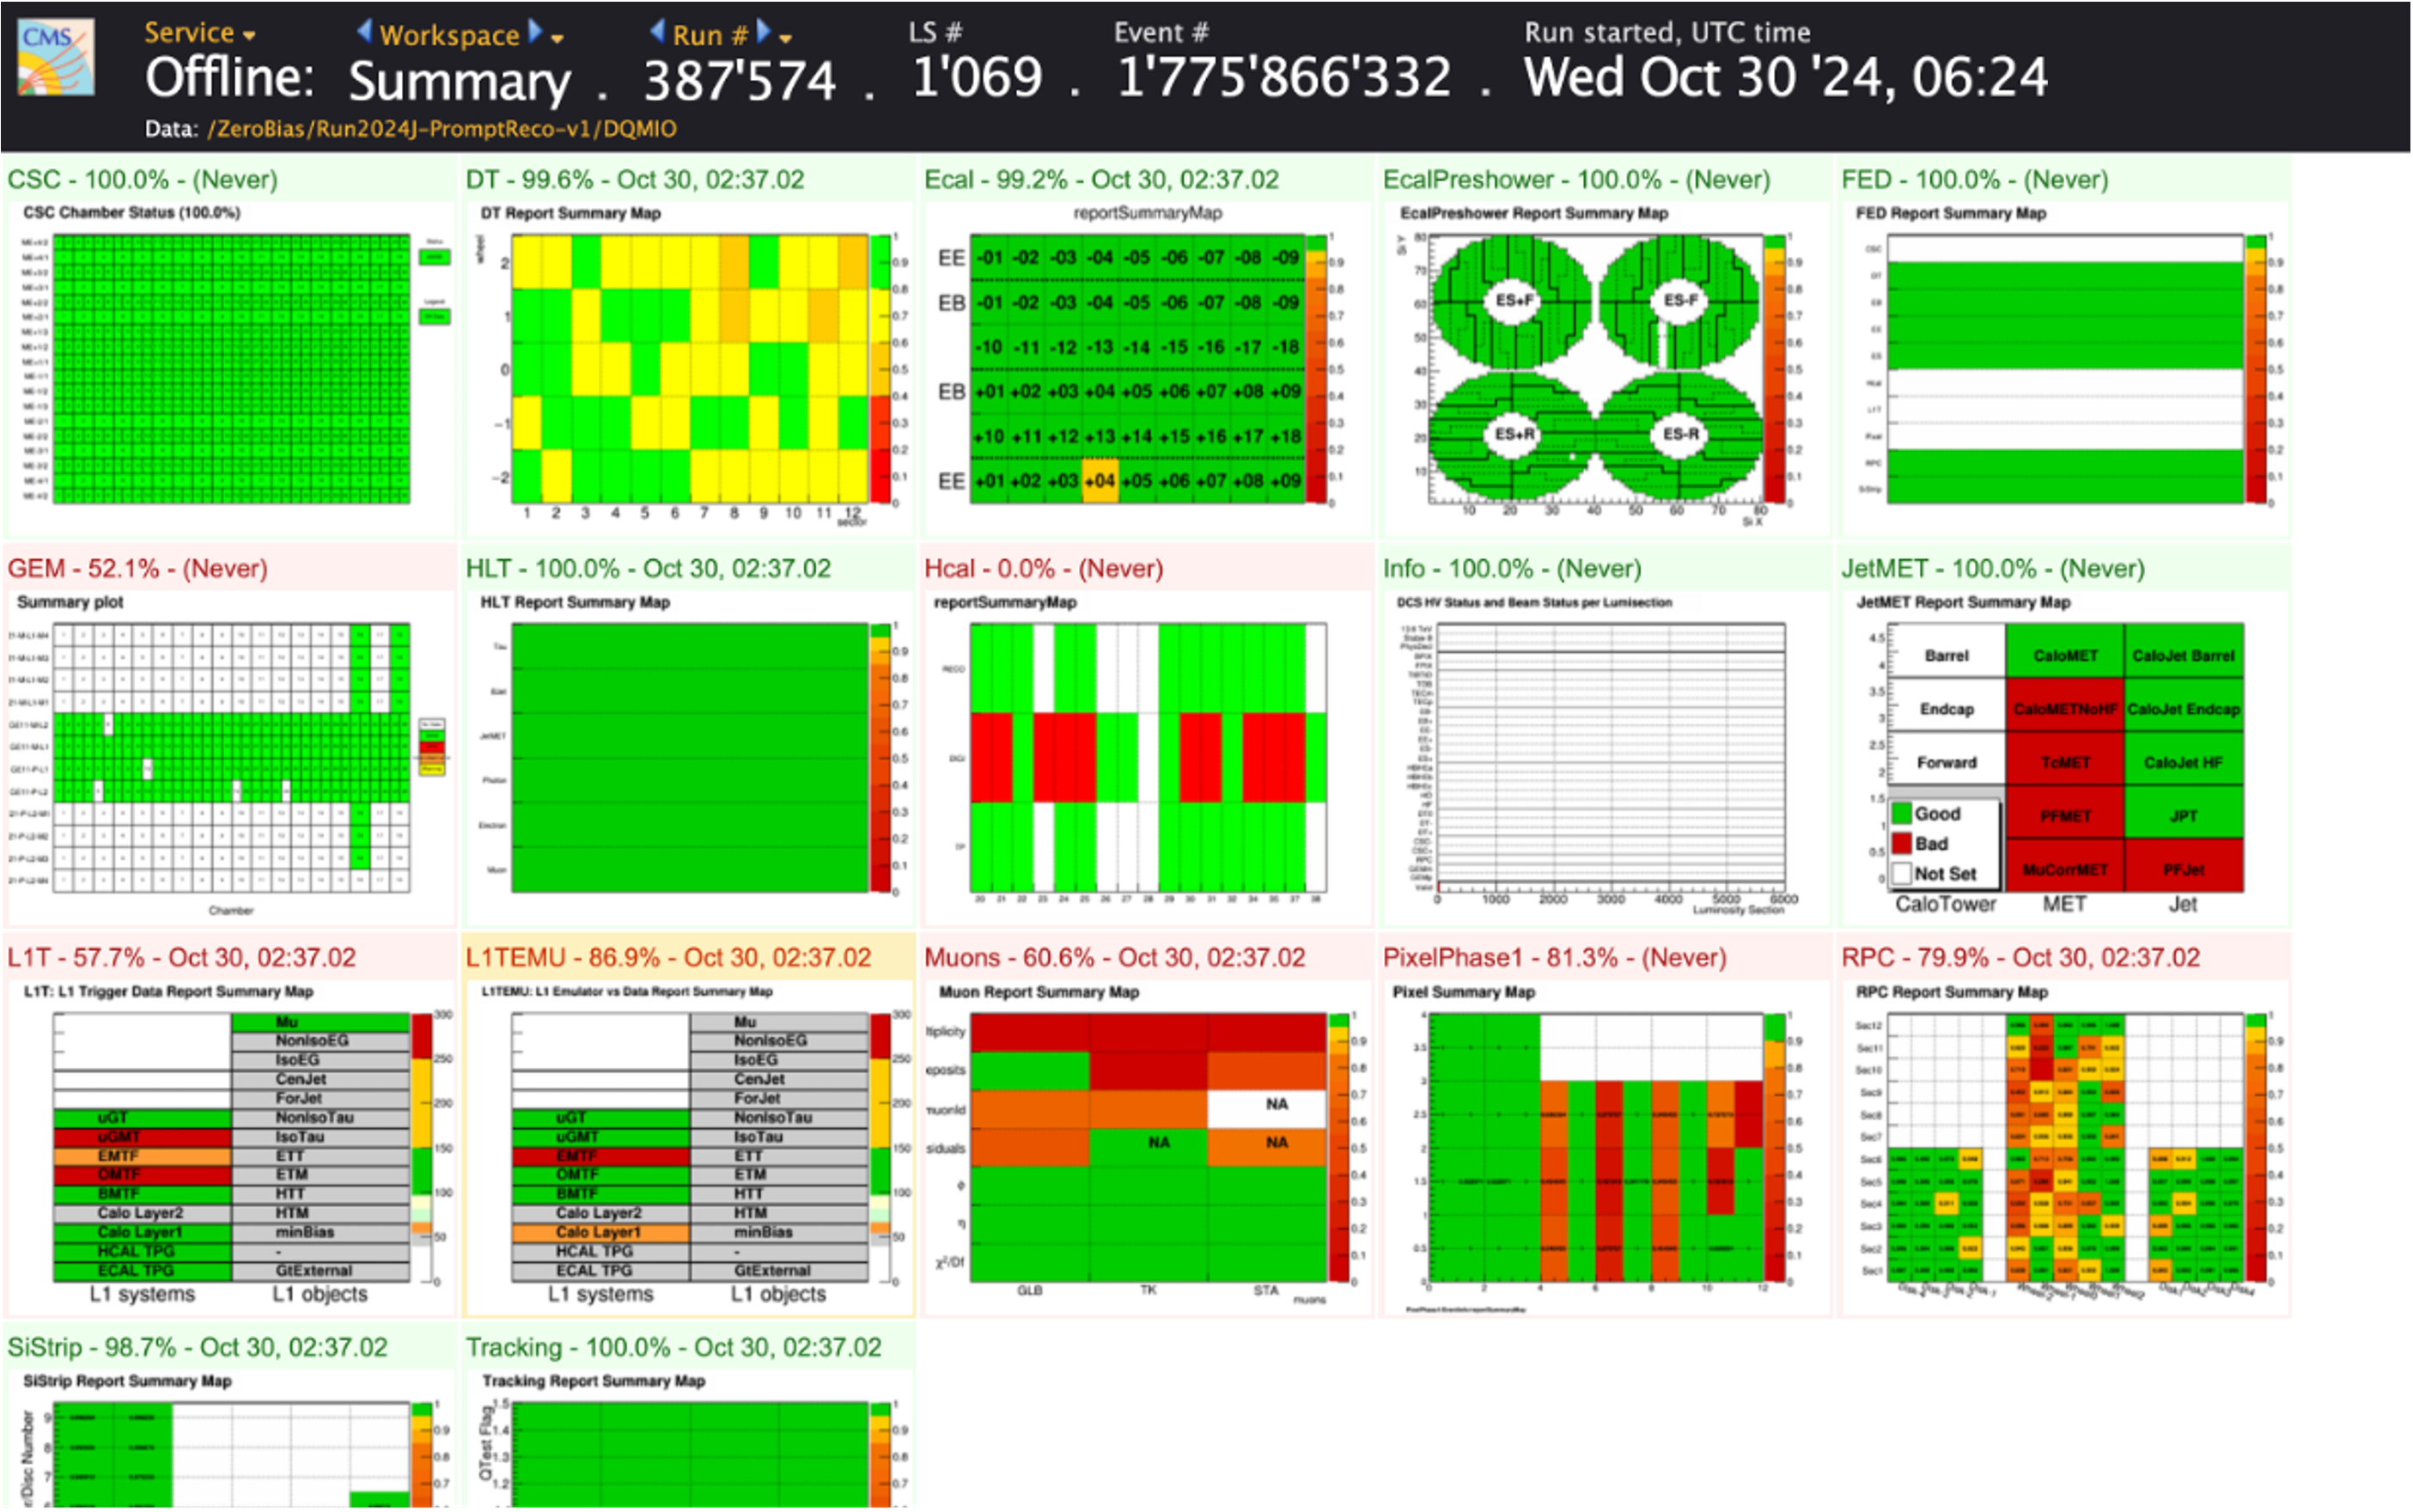
\includegraphics[width=\textwidth]{images/dqm_gui.png}
        \label{fig:dqm_gui_1}
        \caption*{(a)} % Manual label only
    \end{subfigure}

    \vspace{1em}

    \begin{subfigure}[t]{1\textwidth}
        \centering
        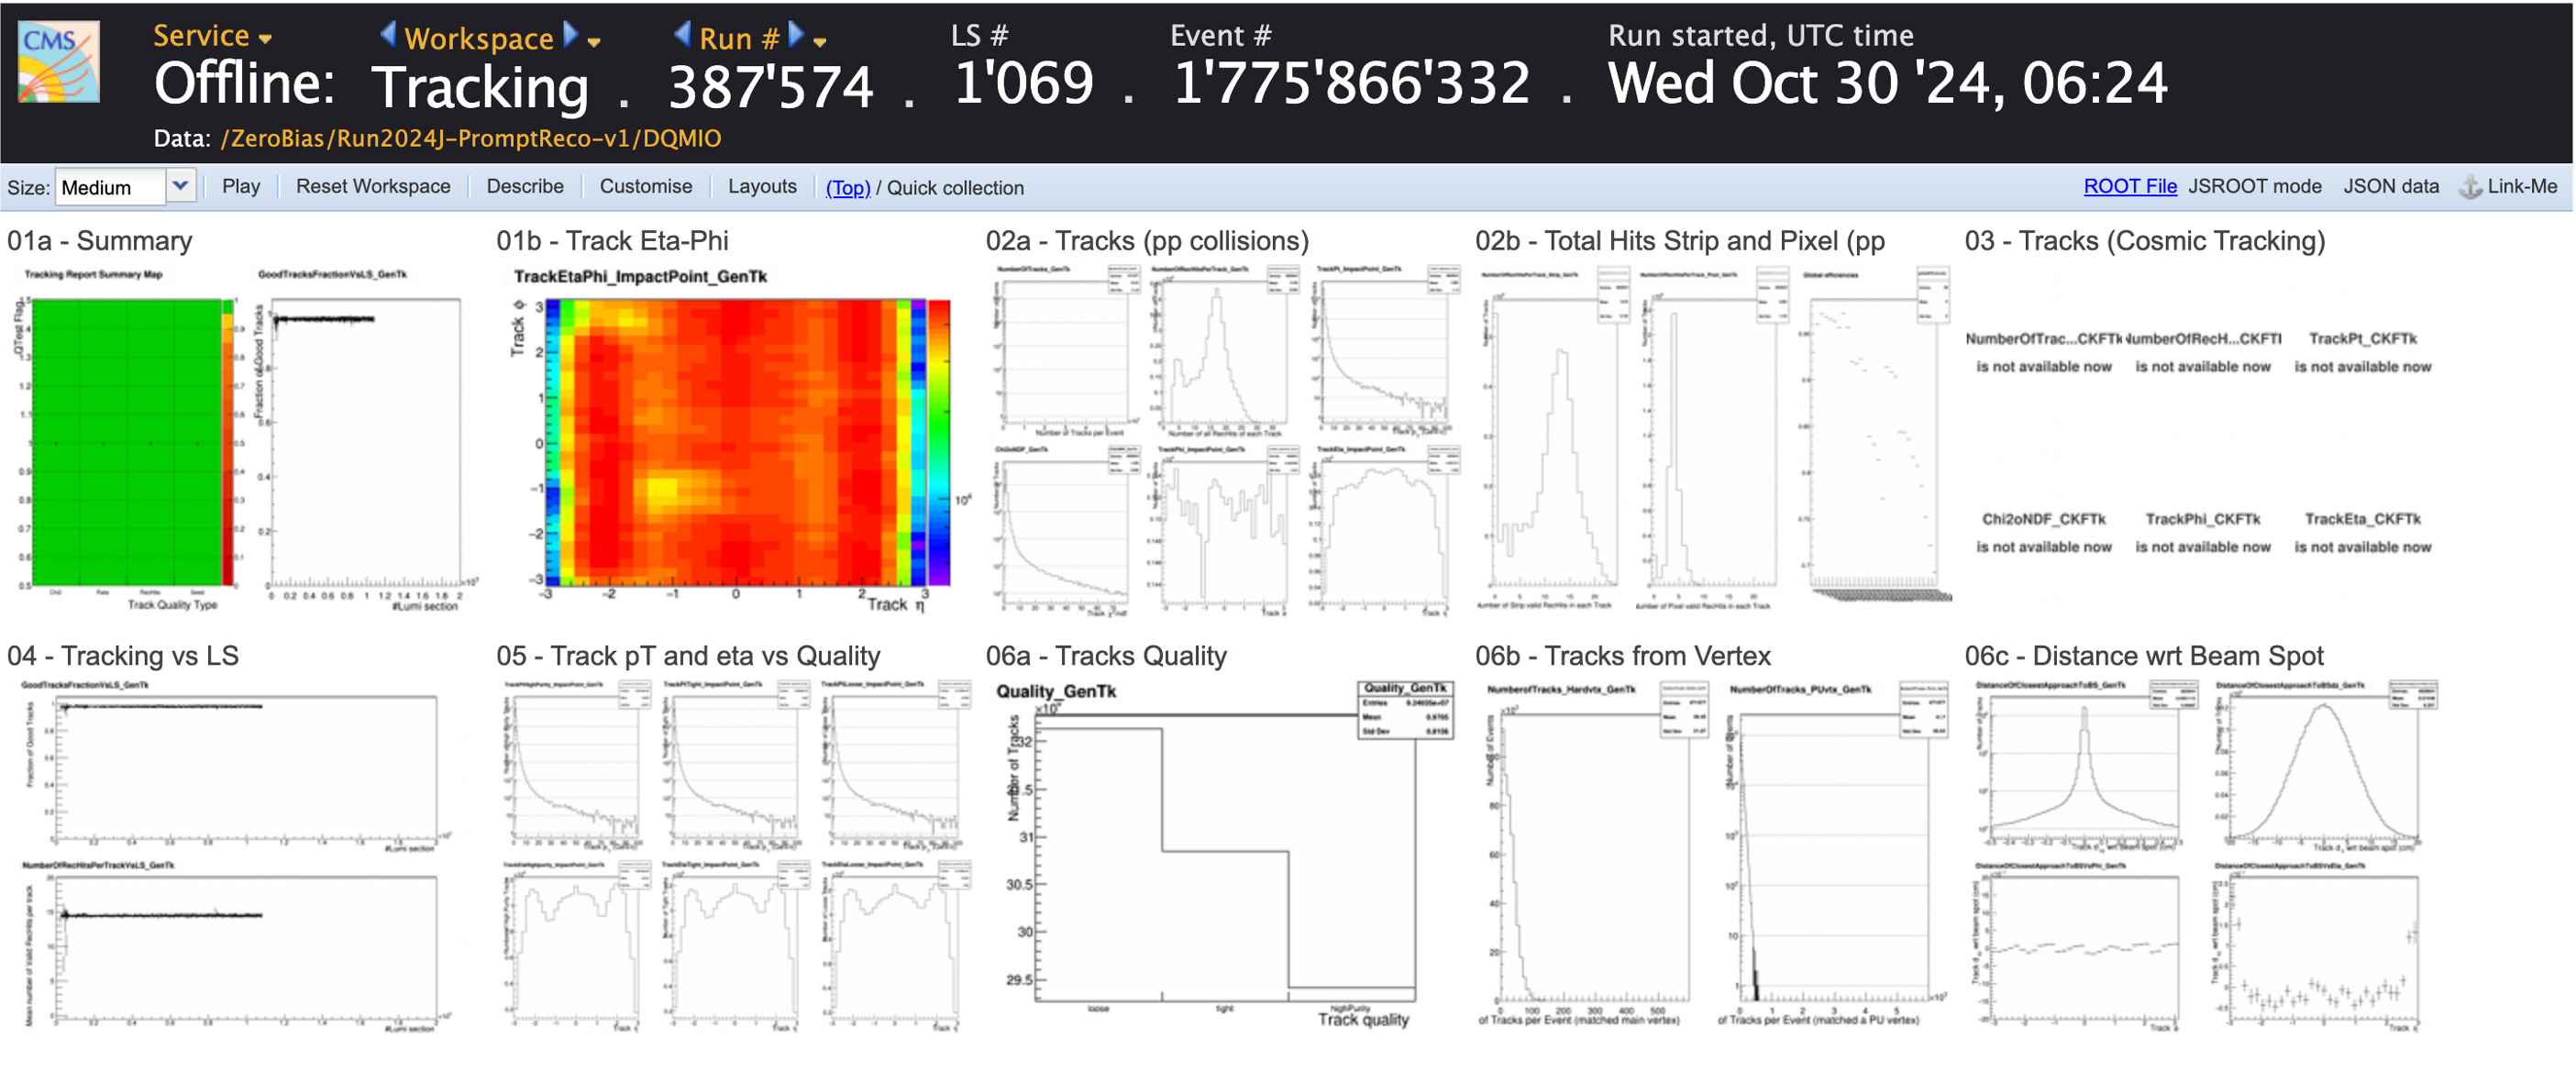
\includegraphics[width=\textwidth]{images/gui_tracker.png}
        \label{fig:dqm_gui_2}
        \caption*{(b)} % Manual label only
    \end{subfigure}

    \caption{A snapshot of the Offline DQM GUI displaying the global summary view (a), and a detailed view of MEs for the tracking system (b).}
    \label{fig:dqm_gui}
\end{figure}
